% !TeX spellcheck = en_US
% !TeX root = notes.tex
\section{Monopoly and Imperfect Competition}
\begin{figure}[H]
	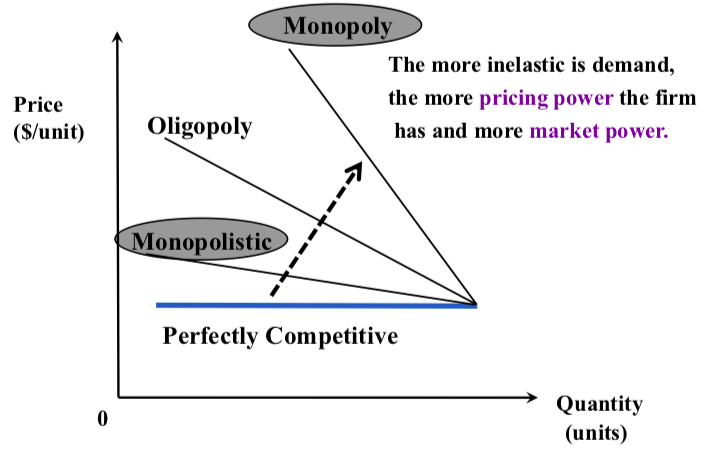
\includegraphics[width=\linewidth]{monopoly}
	\caption{Demand for Perfectly and Imperfectly Competitive Firms}
\end{figure}

\subsection{Perfectly Competitive Firm}
\begin{itemize}
	\item demand is perfectly elastic (horizontal)
	\item is a \textbf{price taker}, maximizing profit where quantity exists so that $P=MC$
\end{itemize}

\subsection{Imperfectly Competitive Firm}
\begin{itemize}
	\item faces a downward sloping demand curve
	\item is a \textbf{price maker}, maximizing profit at a specific output quantity (\textit{not} jsut selling whatever it likes and charging any price!)
\end{itemize}

\subsection{(Pure) Monopoly)}
\begin{note}{Definition}
	\begin{itemize}
		\item a firm that is the \textbf{only} seller of a product or service
		\item it has no \textbf{close} substitutes
		\item the monopoly (firm) supply is the \textbf{market supply}
	\end{itemize}
\end{note}
\subsubsection{Why Monopolies Exist?}
\begin{itemize}
	\item \textbf{Entry} into the industry is \textbf{deliberately blocked} (barriers to entry) allowing only one firm to supply the market
	\item \textbf{Control over key raw material resources} to produce a product
	\item \textbf{Network externalities} = a product's usefulness increase as more consumers adopt it and use it
	\item \textbf{Economies of Scale} (will reduce ATC)
\end{itemize}
\subsubsection{Threat to Monopoly's Existence}
\begin{itemize}
	\item Changes to government legislation (law) to break a monopolies control and power over consumers
	\item The rise of potential competitors who have large amounts of cash, with possibly new improved technologies desired by consumers (evolution of markets)
	\item Economic profits just so high that new entrants are attracted
\end{itemize}
\subsubsection{How does a Monopoly Maximize Profit?}
\begin{align*}
	\text{Marginal Revenue} &= \text{Marginal Cost}\\
	MR&=MC\\
	MR&=\frac{\Delta\text{Revenue}}{\Delta\text{Quantity}}
\end{align*}
\subsubsection{A Profit Maximizing Monopoly}
\begin{itemize}
	\item Taking the ATC curve for a monopoly as U-shaped and demand linear, MC should cut ATC at its minimum
	\item The profit maximizing output quantity can be found where MR and MC intersect
\end{itemize}

\vspace{2em}

\noindent When \textbf{MR} $>$ \textbf{MC} for a given level of output, the firm should \textbf{increase} output to maximize profit. When \textbf{MR} $<$ \textbf{MC} for a given level of output, the firm should \textbf{decrease} output to maximize profits.

\subsubsection{Impacts of Monopoly on Economic Surplus}
\begin{itemize}
	\item Only in perfectly competitive markets, will there be no loss of economic efficiency
	\item In reality, few markets are perfectly competitive, and the MR curve is downward sloping
	\item When $MR = MC$, there will always be some dead weight loss. The closer the price is to MC, the smaller the dead weight loss and inefficiency
	\item The ability to exert \textbf{market power} (how high price can be set price above MC for a given output quantity) dictates the extent of any dead weight loss
\end{itemize}

\subsubsection{Impacts of Market (Pricing) Power}
\textbf{Definition:} A firm that profit maximizes, at an output quantity where \textbf{price} is much larger that \textbf{MC}, is said to have \textbf{Market Power}. For a single supplier, the higher the price is able to be set above MC, the more \textbf{monopoly power}.

\subsubsection{Government Policies to deal with Monopolies}
\begin{itemize}
	\item Monopolies produce economic inefficiencies. Governments aim to improve economic efficiency using \textbf{regulations}
	\item Regulators aim to \textbf{monitor prices} set by monopolies to more closely reflect a \textbf{competitive outcome}
	\item Not only through price regulation, governments can also dictate the quantity to be supplied by monopoly, as well as the timing/amount of any new investments
\end{itemize}

\subsection{The role of the ACCC}
Australian and Consumer Competition Commission (ACCC) = a ``watch dog'' type organisation to monitor competitive behaviour of firms, and to focus on:
\begin{enumerate}
	\item promoting competition, openness and efficiency in the Australian economy
	\item prosecuting firms who breach the Australian Consumer Law 2011 and who engage in anti-competitive and illegal behavior (price fixing, collusion, cartels)
	\item assessing mergers or takeovers for any substantial lessening of competition
\end{enumerate}

\subsection{Monopolistic Competition}
Feature:
\begin{itemize}
	\item A larger number of similar firms exist
	\item Many close substitutes exist
	\item Few barriers to entry into the industry
\end{itemize}
\textit{But} an important difference = \textbf{products/services} can be slightly \textbf{differentiated} (i.e. not identical) giving the firm some pricing power (downward sloping demand)\\
Differentiation the key
\begin{itemize}
	\item some differentiation of product for the firm is possible, allowing the firm some pricing power so the demand curve for the firm is slightly downward sloping
	\item the demand curve for the firm is slightly downward sloping, since a price increase of its product causes a decrease in the quantity demanded by customers. MR will also be downward sloping
\end{itemize}

\subsection{Conclusion}
\begin{itemize}
	\item From \textbf{economist's} view, the existence of a single supplier in the market (monopoly) results in an inefficient allocation of resources (dead weight losses)
	\item From a \textbf{firm's} perspective, resources satisfying opportunities to develop market power, earn economic profits, and increase a firm's value
	\item From a \textbf{government's} view, firms are encouraged to innovate to benefit society, but government regulation is used to limit the extent of the firm's profits
\end{itemize}